\section{Introduction}
\label{sec:introduction}

AI systems increasingly produce candidate updates that may enter persistent operational records. Before admission, an output is a proposal whose origin, context, and uncertainty remain open to inspection. After admission, a value may drive reporting, payment, scheduling, or later automated decisions as a durable fact. The central systems question is therefore not merely whether a model produced a plausible value, but which authority made which value authoritative from which persisted proposal and record state.

Consider a record whose authoritative quantity is 90. A recognizer proposes \code{quantity=100}, but a reviewer authorizes 101; an unchanged batch-code field should retain its earlier source. The value 101 could also result from accepting a machine proposal of 101. These histories have the same final value but different proposal and authorization roles. Rewriting the original candidate would falsely attribute 101 to the model; losing the unchanged field's source would leave the values intact but the lineage incomplete. To reconstruct the correction, admission must retain the predecessor value 90, the proposal $x_c=100$, and the human-authorized value $x_a=101$, allowing
\begin{equation}
x_c\neq x_a
\label{eq:intro-correction}
\end{equation}
while retaining both roles and the exact sources of the complete successor.

This problem arises in systems where people can correct AI-generated field candidates, accepted updates become persistent operational facts, and later review must reconstruct who authorized each value and where it came from. Authorized mutation changes an object that is already authoritative; correction-aware admission additionally preserves the relation between an untrusted proposal, a separate human decision, and the resulting authoritative record.

Existing systems address adjacent layers of this transition. Continuity Kernel separates off-commit candidates from atomic authoritative activation; LatticeMind treats conflict-aware claim selection and supersession as a write-time memory primitive; authority-collapse work studies loss of source authority during memory consolidation; MutMem binds cryptographically authorized changes to predecessor history; and MemTxn provides source-supported update and recovery boundaries \citep{he2026continuity,zhou2026latticemind,zhan2026authoritycollapse,saidi2026mutmem,cui2026memtxn}. Together, these mechanisms establish transaction, provenance, freshness, activation, and governed-memory foundations. This paper isolates correction-aware admission as the unit of analysis: an exact field candidate prompts a human decision that may authorize a different value, after which the system must construct a complete attributable record successor.

We introduce that relation as a correction-aware, field-level specialization of authoritative-state admission. Its semantic chain is
\begin{equation}
\begin{aligned}
\textit{exact candidate}
&\rightarrow\textit{candidate-bound human authorization}\\
&\rightarrow\textit{explicit authorized value}
\rightarrow\textit{complete successor}\\
&\rightarrow\textit{total field-source attribution}.
\end{aligned}
\label{eq:admission-chain}
\end{equation}
The candidate remains non-authoritative historical evidence; the authorization supplies authority for the value; and a trusted transaction constructs the successor. This representation-independent formulation specifies the observable distinctions a mechanism must preserve to separate the failure families considered here.

Five questions organize the characterization: which exact candidate prompted the decision; which value the machine proposed and which value the human authorized; whether the predecessor was still current at admission; whether the declared batch formed one complete successor; and which transition accounts for every changed or unchanged field. Candidate context, value roles, freshness, commit grouping, and total source attribution make these questions observable. The corresponding failure families are candidate substitution, false value attribution, stale replay, fragmented successors, and source ambiguity. We call this the \emph{failure-distinguishability} view of admission.

Our research question is:

\begin{quote}
Which authority-relevant distinctions let a system admit an AI-derived field candidate through an attributable human decision while preserving Correction, freshness, complete-record atomicity, and exact successor lineage?
\end{quote}

The central contribution is the joint relation among proposal identity, human value authority, and complete successor attribution, together with paired histories that expose the consequences of omitting its observation classes. For the 90/100/101 case, these checks distinguish a human correction from model acceptance and preserve the sources of fields left unchanged. We study the relation through \system{}, a Python/SQLite reference realization. C1--C2 specify the contract and its conditional information requirements; C3--C4 provide implementation and evaluation evidence:

\begin{enumerate}[label=\textbf{C\arabic*:},leftmargin=*]
  \item \textbf{Correction-aware admission contract.} The contract keeps the machine's proposal and the human's permitted value separately attributable when $x_c\neq x_a$, binds authorization to the exact candidate, and retains sources for both changed and unchanged fields in one complete successor.
  \item \textbf{Conditional failure-distinguishability characterization.} Five safe/unsafe history pairs show what becomes indistinguishable when each observation class is omitted under the declared model. They connect the contract's information requirements to checks for substitution, false attribution, stale replay, fragmented commits, and source ambiguity.
  \item \textbf{Relational and transactional realization.} We connect the contract to bounded Alloy assertions and encoding-sensitivity checks, a compare-and-swap-protected transaction, selected formal--concrete projections, and a production-facing fault catalogue.
  \item \textbf{Cost and agent-integration evaluation.} We measure persistence-equivalent admission costs and trace access, then evaluate a restricted proposal/verification surface across three qualified model configurations. Agent completion, acknowledgment, and recovery are assessed separately from host-enforced authority outcomes.
\end{enumerate}

The evaluation follows three questions in this dependency chain: which information is needed to distinguish admission failures (RQ1--RQ2), whether the transaction preserves these relations in persisted executions (RQ3--RQ5), and what costs and agent-integration behavior arise in the reference realization (RQ6--RQ8). \Cref{fig:admission-workflow} gives an overview of the proposal, review, and admission boundary.

% FIGURE SOURCE: scripts/build_flowcharts.py; vector redraw preserving the author-approved workflow semantics.
\begin{figure*}[t]
\centering
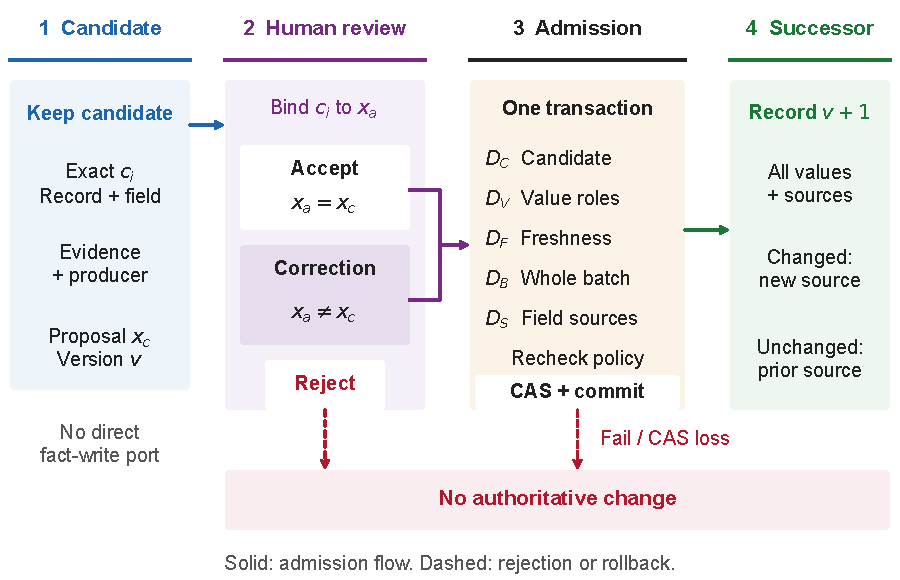
\includegraphics[width=0.96\textwidth]{figures/refined/figure-1-admission-workflow.pdf}
\caption{Correction-aware authoritative-state admission. Only candidate-bound Accept or Correction decisions proceed to transactional admission. The declared distinction checks, host-policy revalidation, and version compare-and-swap protect creation of a complete successor and total source map. Reject, failed validation, or a lost compare-and-swap leaves authoritative state unchanged. Authorization records responsibility, not factual truth.}
\label{fig:admission-workflow}
\end{figure*}

The remainder of the paper positions the abstraction against its nearest neighbors (\cref{sec:related}), defines the observation model and admission contract (\cref{sec:contract}), presents the bounded and concrete realizations (\cref{sec:alloy,sec:realization}), explains their selected correspondence (\cref{sec:conformance}), and reports the evaluation (\cref{sec:evaluation,sec:results}) before discussing inference boundaries (\cref{sec:discussion}).
